\hypertarget{einleitung}{%
\section{Einleitung}\label{einleitung}}

\hypertarget{motivation}{%
\subsection{Motivation}\label{motivation}}

\begin{itemize}
\tightlist
\item
  Beginn: Er zieht die Aufmerksamkeit des Lesers durch die Schilderung
  des Ereignisses auf sich, das zu dem Problem geführt hat.
\item
  Hintergrundinformationen (Herstellung des Kontexts): Gehe tiefer auf
  das Ereignis ein, indem du mehr Informationen über es vermittelst und
  dabei auch den Rahmen deiner Forschung skizzierst.
\item
  Brücke zur Problemstellung: Erläutere, inwiefern es sich hierbei um
  ein Problem handelt, und schlage somit die Brücke zur Problemstellung,
  die deiner Untersuchung zu Grunde liegt.
\end{itemize}

\hypertarget{zielsetzung}{%
\subsection{Zielsetzung}\label{zielsetzung}}

Das Ziel dieser Arbeit ist es, einen autonomen Schach-Tisch, welcher in
der Lage ist Schachfiguren autonom zu bewegen und auf
Benutzerinteraktion zu reagieren.

Der Schwerpunkt liegt dabei insbesondere auf der Programmierung des
eingebettenen Systems. Dieses besteht zum einem, aus der
Positionserkennung und Steuerung der Hardwarekomponenten (Schachfiguren)
und zum anderen aus der Kommunikation zwischen dem Tisch selbst und
einem in einer Cloud befindlichen Server.

Mittels der Programmierung werden diverse Technologien von verschiedenen
Einzelsystemen zu einem Gesamtprodukt zusammengesetzt. Zu diesen
Einzelsystemen gehören:

\begin{itemize}
\tightlist
\item
  Programmierung der Motorsteuerung, HMI (zB. Qt oder simple Buttons),
  NFC Tag erkennung
\item
  Programmierung eines Wrappers für die Kommunikation mit der Cloud
  (AWS)
\item
  Statemaschiene und Implementierung der Spielflusssteuerung
\item
  Backend mit Datenbankanbindung zwischen Server und Embedded-System
\item
  Verwendung eines CI/CD Systems zum automatisierten bauen der
  Linux-Images für das Embedded-System
\end{itemize}

\hypertarget{aufbau-der-arbeit}{%
\subsection{Aufbau der Arbeit}\label{aufbau-der-arbeit}}

beleuchtung existierender ansätze \&\& festlegung zu erwartener
Features, Kapitel x+1 zusammenführung in die DK HW,Kaptiel x+4 test und
fazit,demonstration und validierung der funktionsfähigkeit

\hypertarget{analyse-bestehender-systeme-und-machbarkeitsanalyse}{%
\section{Analyse bestehender Systeme und
Machbarkeitsanalyse}\label{analyse-bestehender-systeme-und-machbarkeitsanalyse}}

\hypertarget{existierende-systeme-im-vergleich}{%
\subsection{Existierende Systeme im
Vergleich}\label{existierende-systeme-im-vergleich}}

\hypertarget{kommerzielle-produkte}{%
\subsubsection{Kommerzielle Produkte}\label{kommerzielle-produkte}}

\begin{itemize}
\tightlist
\item
  zwei hersteller wirklich autonomer schachtische; für tunieren werden
  dgt schachbretter für livestreams und recordinge verwendet.
\end{itemize}

\begin{longtable}[]{@{}lllll@{}}
\caption{Auflistung kommerzieller autonomer Schachtische}\tabularnewline
\toprule
\begin{minipage}[b]{0.18\columnwidth}\raggedright
\strut
\end{minipage} & \begin{minipage}[b]{0.18\columnwidth}\raggedright
Square Off - Kingdom \autocite{squareoffkingdom}\strut
\end{minipage} & \begin{minipage}[b]{0.22\columnwidth}\raggedright
Square Off - Grand Kingdom \autocite{squareoffgrand}\strut
\end{minipage} & \begin{minipage}[b]{0.15\columnwidth}\raggedright
DGT Smart Board \autocite{dtgsmartboard}\strut
\end{minipage} & \begin{minipage}[b]{0.13\columnwidth}\raggedright
DGT Bluetooth Wenge \autocite{dtgble}\strut
\end{minipage}\tabularnewline
\midrule
\endfirsthead
\toprule
\begin{minipage}[b]{0.18\columnwidth}\raggedright
\strut
\end{minipage} & \begin{minipage}[b]{0.18\columnwidth}\raggedright
Square Off - Kingdom \autocite{squareoffkingdom}\strut
\end{minipage} & \begin{minipage}[b]{0.22\columnwidth}\raggedright
Square Off - Grand Kingdom \autocite{squareoffgrand}\strut
\end{minipage} & \begin{minipage}[b]{0.15\columnwidth}\raggedright
DGT Smart Board \autocite{dtgsmartboard}\strut
\end{minipage} & \begin{minipage}[b]{0.13\columnwidth}\raggedright
DGT Bluetooth Wenge \autocite{dtgble}\strut
\end{minipage}\tabularnewline
\midrule
\endhead
\begin{minipage}[t]{0.18\columnwidth}\raggedright
Erkennung Schachfigurstellung\strut
\end{minipage} & \begin{minipage}[t]{0.18\columnwidth}\raggedright
nein (Manuell per Ausgangsposition)\strut
\end{minipage} & \begin{minipage}[t]{0.22\columnwidth}\raggedright
nein (Manuell per Ausgangsposition)\strut
\end{minipage} & \begin{minipage}[t]{0.15\columnwidth}\raggedright
ja (Resonanzspulen)\strut
\end{minipage} & \begin{minipage}[t]{0.13\columnwidth}\raggedright
ja (\gls{rfid})\strut
\end{minipage}\tabularnewline
\begin{minipage}[t]{0.18\columnwidth}\raggedright
Tischabmessungen (LxBxH)\strut
\end{minipage} & \begin{minipage}[t]{0.18\columnwidth}\raggedright
486mm x 486mm x 75mm\strut
\end{minipage} & \begin{minipage}[t]{0.22\columnwidth}\raggedright
671mm x 486mm x 75mm\strut
\end{minipage} & \begin{minipage}[t]{0.15\columnwidth}\raggedright
540mm x 540mm x 20mm\strut
\end{minipage} & \begin{minipage}[t]{0.13\columnwidth}\raggedright
540mm x 540mm x 20mm\strut
\end{minipage}\tabularnewline
\begin{minipage}[t]{0.18\columnwidth}\raggedright
Konnektivität\strut
\end{minipage} & \begin{minipage}[t]{0.18\columnwidth}\raggedright
\gls{ble}\strut
\end{minipage} & \begin{minipage}[t]{0.22\columnwidth}\raggedright
\gls{ble}\strut
\end{minipage} & \begin{minipage}[t]{0.15\columnwidth}\raggedright
\gls{usb} / Seriell\strut
\end{minipage} & \begin{minipage}[t]{0.13\columnwidth}\raggedright
Bluetooth 2.0\strut
\end{minipage}\tabularnewline
\begin{minipage}[t]{0.18\columnwidth}\raggedright
Automatisches Bewegen der Figuren\strut
\end{minipage} & \begin{minipage}[t]{0.18\columnwidth}\raggedright
ja\strut
\end{minipage} & \begin{minipage}[t]{0.22\columnwidth}\raggedright
ja\strut
\end{minipage} & \begin{minipage}[t]{0.15\columnwidth}\raggedright
nein\strut
\end{minipage} & \begin{minipage}[t]{0.13\columnwidth}\raggedright
nein\strut
\end{minipage}\tabularnewline
\begin{minipage}[t]{0.18\columnwidth}\raggedright
Spiel Livestream\strut
\end{minipage} & \begin{minipage}[t]{0.18\columnwidth}\raggedright
ja\strut
\end{minipage} & \begin{minipage}[t]{0.22\columnwidth}\raggedright
ja\strut
\end{minipage} & \begin{minipage}[t]{0.15\columnwidth}\raggedright
ja\strut
\end{minipage} & \begin{minipage}[t]{0.13\columnwidth}\raggedright
ja\strut
\end{minipage}\tabularnewline
\begin{minipage}[t]{0.18\columnwidth}\raggedright
Cloud anbindung (online Spiele)\strut
\end{minipage} & \begin{minipage}[t]{0.18\columnwidth}\raggedright
ja (über Mobiltelefon + App)\strut
\end{minipage} & \begin{minipage}[t]{0.22\columnwidth}\raggedright
ja (über Mobiltelefon + App)\strut
\end{minipage} & \begin{minipage}[t]{0.15\columnwidth}\raggedright
ja (über PC + App)\strut
\end{minipage} & \begin{minipage}[t]{0.13\columnwidth}\raggedright
ja (über PC + App)\strut
\end{minipage}\tabularnewline
\begin{minipage}[t]{0.18\columnwidth}\raggedright
Parkposition für ausgeschiedene Figuren\strut
\end{minipage} & \begin{minipage}[t]{0.18\columnwidth}\raggedright
nein\strut
\end{minipage} & \begin{minipage}[t]{0.22\columnwidth}\raggedright
ja\strut
\end{minipage} & \begin{minipage}[t]{0.15\columnwidth}\raggedright
nein\strut
\end{minipage} & \begin{minipage}[t]{0.13\columnwidth}\raggedright
nein\strut
\end{minipage}\tabularnewline
\begin{minipage}[t]{0.18\columnwidth}\raggedright
Stand-Alone Funktionalität\strut
\end{minipage} & \begin{minipage}[t]{0.18\columnwidth}\raggedright
nein (Mobiltelefon erforderlich)\strut
\end{minipage} & \begin{minipage}[t]{0.22\columnwidth}\raggedright
nein (Mobiltelefon erforderlich)\strut
\end{minipage} & \begin{minipage}[t]{0.15\columnwidth}\raggedright
nein (PC erforderlich)\strut
\end{minipage} & \begin{minipage}[t]{0.13\columnwidth}\raggedright
nein (PC erforderlich)\strut
\end{minipage}\tabularnewline
\begin{minipage}[t]{0.18\columnwidth}\raggedright
Besonderheiten\strut
\end{minipage} & \begin{minipage}[t]{0.18\columnwidth}\raggedright
Akku für 30 Spiele\strut
\end{minipage} & \begin{minipage}[t]{0.22\columnwidth}\raggedright
Akku für 15 Spiele\strut
\end{minipage} & \begin{minipage}[t]{0.15\columnwidth}\raggedright
-\strut
\end{minipage} & \begin{minipage}[t]{0.13\columnwidth}\raggedright
-\strut
\end{minipage}\tabularnewline
\bottomrule
\end{longtable}

\hypertarget{open-source-projekte}{%
\subsubsection{Open-Source Projekte}\label{open-source-projekte}}

Bei allen Open-Source Projekten wurden die Features anhand der
Beschreibung und der aktuellen Software extrahiert. Besonders bei
work-in-progress Projekten können sich die Features noch verändern und
so weitere Funktionalitäten hinzugefügt werden.

Des Weiteren gibt es weitere derartige Projekte, in der Tabelle wurde
nur diese Aufgelistet welche sich von anderen Projekten in mindestens
einem Feature unterscheiden.

Auch existieren weitere Abwandlungen von autonomen Schachbrettern, bei
welchem die Figuren von oberhalb des Spielbretts gegriffen bzw. bewegt
werden. In einigen Projekten wird dies mittels eines Industrie-Roboters
\autocite{actprojectrobot} oder eines modifizierten
3D-Druckers\autocite{atcproject3dprinter} realisiert, diese wurden hier
nicht aufgrund der Mechanik welche über dem Spielbrett montiert werden
muss nicht berücksichtigt.

\begin{longtable}[]{@{}llll@{}}
\caption{Auflistung von Open-Source Schachtisch
Projekten}\tabularnewline
\toprule
\begin{minipage}[b]{0.20\columnwidth}\raggedright
\strut
\end{minipage} & \begin{minipage}[b]{0.24\columnwidth}\raggedright
Automated Chess Board (Michael Guerero) \autocite{actproject1}\strut
\end{minipage} & \begin{minipage}[b]{0.26\columnwidth}\raggedright
Automated Chess Board (Akash Ravichandran) \autocite{actproject2}\strut
\end{minipage} & \begin{minipage}[b]{0.19\columnwidth}\raggedright
DIY Super Smart Chessboard \autocite{actproject3}\strut
\end{minipage}\tabularnewline
\midrule
\endfirsthead
\toprule
\begin{minipage}[b]{0.20\columnwidth}\raggedright
\strut
\end{minipage} & \begin{minipage}[b]{0.24\columnwidth}\raggedright
Automated Chess Board (Michael Guerero) \autocite{actproject1}\strut
\end{minipage} & \begin{minipage}[b]{0.26\columnwidth}\raggedright
Automated Chess Board (Akash Ravichandran) \autocite{actproject2}\strut
\end{minipage} & \begin{minipage}[b]{0.19\columnwidth}\raggedright
DIY Super Smart Chessboard \autocite{actproject3}\strut
\end{minipage}\tabularnewline
\midrule
\endhead
\begin{minipage}[t]{0.20\columnwidth}\raggedright
Erkennung Schachfigurstellung\strut
\end{minipage} & \begin{minipage}[t]{0.24\columnwidth}\raggedright
nein (Manuell per Ausgangsposition)\strut
\end{minipage} & \begin{minipage}[t]{0.26\columnwidth}\raggedright
ja (Kamera / OpenCV)\strut
\end{minipage} & \begin{minipage}[t]{0.19\columnwidth}\raggedright
nein\strut
\end{minipage}\tabularnewline
\begin{minipage}[t]{0.20\columnwidth}\raggedright
Tischabmessungen (LxBxH)\strut
\end{minipage} & \begin{minipage}[t]{0.24\columnwidth}\raggedright
keine Angabe\strut
\end{minipage} & \begin{minipage}[t]{0.26\columnwidth}\raggedright
keine Angabe\strut
\end{minipage} & \begin{minipage}[t]{0.19\columnwidth}\raggedright
450mm x 300mm x 50mm\strut
\end{minipage}\tabularnewline
\begin{minipage}[t]{0.20\columnwidth}\raggedright
Konnektivität\strut
\end{minipage} & \begin{minipage}[t]{0.24\columnwidth}\raggedright
\gls{usb}\strut
\end{minipage} & \begin{minipage}[t]{0.26\columnwidth}\raggedright
Ethernet, \gls{wlan}\strut
\end{minipage} & \begin{minipage}[t]{0.19\columnwidth}\raggedright
Ethernet, \gls{wlan}\strut
\end{minipage}\tabularnewline
\begin{minipage}[t]{0.20\columnwidth}\raggedright
Automatisches Bewegen der Figuren\strut
\end{minipage} & \begin{minipage}[t]{0.24\columnwidth}\raggedright
ja\strut
\end{minipage} & \begin{minipage}[t]{0.26\columnwidth}\raggedright
ja\strut
\end{minipage} & \begin{minipage}[t]{0.19\columnwidth}\raggedright
nein\strut
\end{minipage}\tabularnewline
\begin{minipage}[t]{0.20\columnwidth}\raggedright
Spiel Livestream\strut
\end{minipage} & \begin{minipage}[t]{0.24\columnwidth}\raggedright
nein\strut
\end{minipage} & \begin{minipage}[t]{0.26\columnwidth}\raggedright
nein\strut
\end{minipage} & \begin{minipage}[t]{0.19\columnwidth}\raggedright
nein\strut
\end{minipage}\tabularnewline
\begin{minipage}[t]{0.20\columnwidth}\raggedright
Cloud anbindung (online Spiele)\strut
\end{minipage} & \begin{minipage}[t]{0.24\columnwidth}\raggedright
nein\strut
\end{minipage} & \begin{minipage}[t]{0.26\columnwidth}\raggedright
nein\strut
\end{minipage} & \begin{minipage}[t]{0.19\columnwidth}\raggedright
ja\strut
\end{minipage}\tabularnewline
\begin{minipage}[t]{0.20\columnwidth}\raggedright
Parkposition für ausgeschiedene Figuren\strut
\end{minipage} & \begin{minipage}[t]{0.24\columnwidth}\raggedright
nein\strut
\end{minipage} & \begin{minipage}[t]{0.26\columnwidth}\raggedright
nein\strut
\end{minipage} & \begin{minipage}[t]{0.19\columnwidth}\raggedright
nein\strut
\end{minipage}\tabularnewline
\begin{minipage}[t]{0.20\columnwidth}\raggedright
Stand-Alone Funktionalität\strut
\end{minipage} & \begin{minipage}[t]{0.24\columnwidth}\raggedright
nein (PC erforderlich)\strut
\end{minipage} & \begin{minipage}[t]{0.26\columnwidth}\raggedright
ja\strut
\end{minipage} & \begin{minipage}[t]{0.19\columnwidth}\raggedright
ja\strut
\end{minipage}\tabularnewline
\begin{minipage}[t]{0.20\columnwidth}\raggedright
Besonderheiten\strut
\end{minipage} & \begin{minipage}[t]{0.24\columnwidth}\raggedright
-\strut
\end{minipage} & \begin{minipage}[t]{0.26\columnwidth}\raggedright
Sprachsteuerung (Amazon Alexa)\strut
\end{minipage} & \begin{minipage}[t]{0.19\columnwidth}\raggedright
Zuganzeige über LED Matrix\strut
\end{minipage}\tabularnewline
\begin{minipage}[t]{0.20\columnwidth}\raggedright
Lizenz\strut
\end{minipage} & \begin{minipage}[t]{0.24\columnwidth}\raggedright
\gls{gpl} 3+\strut
\end{minipage} & \begin{minipage}[t]{0.26\columnwidth}\raggedright
\gls{gpl}\strut
\end{minipage} & \begin{minipage}[t]{0.19\columnwidth}\raggedright
-\strut
\end{minipage}\tabularnewline
\bottomrule
\end{longtable}

In den bestehenden Projekten ist zu erkennen, dass ein autonomer
Schachtisch sehr einfach und mit einfachsten Mittel konstruiert werden
kann. Hierbei fehlen in der Regel einige Features wie das automatische
Erkennen von Figuren oder das Spielen über das Internet.

Einige Projekte setzten dabei auf eingebettete Systeme, welche direkt im
Schachtisch montiert sind, andere hingegen nutzen einen externen PC,
welcher die Steuerbefehle an die Elektronik sendet.

Bei der Konstruktion der Mechanik und der Methode mit welcher die
Figuren über das Feld bewegt werden ähneln sich jedoch die meisten
dieser Projekte. Hier wird meist eine einfache X und Y-Achse verwendet,
welche von zwei Schrittmotoren bewegt werden. Die Schachfiguren werden
dabei mittels eines Elektromagneten über die Oberseite gezogen. Hierbei
ist ein Magnet oder eine kleine Metallplatte in den Fuß der Figuren
eingelassen worden.

Die Erkennung der Schachfiguren ist augenscheinlich die schwierigste
Aufgabe. Hier wurde in der Mehrzahl der Projekte eine Kamera im
Zusammenspiel mit einer auf OpenCV basierenden Figur-Erkennung. Diese
Variante ist je nach Implementierung des Vision-Algorithmus
fehleranfälliger bei sich ändernden Lichtverhältnissen, auch muss die
Kamera oberhalb der Schachfiguren platziert werden, wenn kein
transparentes Schachfeld verwendet werden soll.

\hypertarget{user-experience}{%
\subsection{User Experience}\label{user-experience}}

Ein wichtiger Aspekt bei diesem Projekt spiel die User-Experience. Diese
beschreibt die Ergonomie der Mensch-Maschine Interaktion und wird durch
die DIN 9241\autocite{din9241} beschrieben. Hierbei geht es primär um
das Erlebnis, welches der Benutzer bei dem Verwenden eines Produktes
erlebt und welche Erwartungen der Benutzer an die Verwendung des
Produktes hat.

Bei dem autonomen Schachtisch, soll der Benutzer eine ähnlich einfache
Erfahrung erleben, wie bei einer Schachpartie mit einem menschlichen
Gegenspieler. Der Benutzer soll direkt nach dem einschalten des Tisches
und dem Aufstellen der Figuren in der Lage sein, mit dem Spiel beginnen
zu können. Dies soll wie ein reguläres Schachspiel ablaufen, der Spieler
vor dem Tisch soll die Figuren mit der Hand bewegen können und der Tisch
soll den Gegenspieler darstellen. Dieser bewegt die Figuren der
Gegenseite.

Nach Beendigung einer Partie, soll das Spielbrett wieder in die
Ausgangssituation gebracht werden, die kann zum einem vom Tisch selber
oder vom Benutzer per Hand geschehen. Danach ist der Tisch für die
nächste Partie bereit, welche einfach per Knopfdruck gestartet werden
können sollte.

Ein weiter Punkt welcher bei der User-Experience beachtet werden soll,
ist die zeitliche Konstante. Ein Spiel auf einem normalen Schachspiel
hat je nach Spielart kein Zeitlimit, dies kann für das gesamte Spiel
gelten oder auch für die Zeit zwischen einzelnen Zügen. Der autonome
Schachtisch soll es dem Spieler z.B. ermöglichen ein Spiel am Morgen zu
beginnen und erst am nächsten Tag dieses fortzusetzen.

\hypertarget{anforderungsanalyse}{%
\subsection{Anforderungsanalyse}\label{anforderungsanalyse}}

alle key requirements welcher der tisch haben soll

\hypertarget{machbarkeitsanalyse}{%
\subsection{Machbarkeitsanalyse}\label{machbarkeitsanalyse}}

welche technologien werden benötigt

\hypertarget{technologien-im-makerspace}{%
\subsubsection{Technologien im
Makerspace}\label{technologien-im-makerspace}}

stehen diese im makerspace zur verfüfung

\hypertarget{section}{%
\subsubsection{}\label{section}}

\hypertarget{erstellung-erster-prototyp}{%
\section{Erstellung erster Prototyp}\label{erstellung-erster-prototyp}}

\hypertarget{technologieauswahl-fuxfcr-ersten-protoypen}{%
\subsection{Technologieauswahl für ersten
Protoypen}\label{technologieauswahl-fuxfcr-ersten-protoypen}}

\hypertarget{section-1}{%
\section{}\label{section-1}}

\hypertarget{vinaque-sanguine-metuenti-cuiquam-alcyone-fixus}{%
\section{Vinaque sanguine metuenti cuiquam Alcyone
fixus}\label{vinaque-sanguine-metuenti-cuiquam-alcyone-fixus}}

\hypertarget{aesculeae-domus-vincemur-et-veneris-adsuetus-lapsum}{%
\subsection{Aesculeae domus vincemur et Veneris adsuetus
lapsum}\label{aesculeae-domus-vincemur-et-veneris-adsuetus-lapsum}}

Lorem markdownum Letoia, et alios: figurae flectentem annis aliquid
Peneosque ab esse, obstat gravitate. Obscura atque coniuge, per de
coniunx, sibi \textbf{medias commentaque virgine} anima tamen comitemque
petis, sed. In Amphion vestros hamos ire arceor mandere spicula, in
licet aliquando.

\begin{lstlisting}[language=Java]
public class Example implements LoremIpsum {
    public static void main(String[] args) {
        if(args.length < 2) {
            System.out.println("Lorem ipsum dolor sit amet");
        }
    } // Obscura atque coniuge, per de coniunx
}
\end{lstlisting}

Listing: TEST

\begin{lstlisting}[language={C++}]
// Your First C++ Program

#include <iostream>

int main() {
    std::cout << "Hello World!";
    return 0;
}

}
\end{lstlisting}

Porrigitur et Pallas nuper longusque cratere habuisse sepulcro pectore
fertur. Laudat ille auditi; vertitur iura tum nepotis causa; motus. Diva
virtus! Acrota destruitis vos iubet quo et classis excessere Scyrumve
spiro subitusque mente Pirithoi abstulit, lapides.

\hypertarget{lydia-caelo-recenti-haerebat-lacerum-ratae-at}{%
\subsection{Lydia caelo recenti haerebat lacerum ratae
at}\label{lydia-caelo-recenti-haerebat-lacerum-ratae-at}}

Te concepit pollice fugit vias alumno \textbf{oras} quam potest
\href{http://example.com\#rursus}{rursus} optat. Non evadere orbem
equorum, spatiis, vel pede inter si.

\begin{enumerate}
\def\labelenumi{\arabic{enumi}.}
\tightlist
\item
  De neque iura aquis
\item
  Frangitur gaudia mihi eo umor terrae quos
\item
  Recens diffudit ille tantum
\end{enumerate}

\begin{equation}\label{eq:neighbor-propability}
    p_{ij}(t) = \frac{\ell_j(t) - \ell_i(t)}{\sum_{k \in N_i(t)}^{} \ell_k(t) - \ell_i(t)}
\end{equation}

Tamen condeturque saxa Pallorque num et ferarum promittis inveni lilia
iuvencae adessent arbor. Florente perque at condeturque saxa et ferarum
promittis tendebat. Armos nisi obortas refugit me.

\begin{quote}
Et nepotes poterat, se qui. Euntem ego pater desuetaque aethera
Maeandri, et \href{http://example.com\#Dardanio_geminaque}{Dardanio
geminaque} cernit. Lassaque poenas nec, manifesta \(\pi r^2\) mirantia
captivarum prohibebant scelerato gradus unusque dura.
\end{quote}

\begin{itemize}
\tightlist
\item
  Permulcens flebile simul
\item
  Iura tum nepotis causa motus diva virtus Acrota. Tamen condeturque
  saxa Pallorque num et ferarum promittis inveni lilia iuvencae adessent
  arbor. Florente perque at ire arcum.
\end{itemize}

\hypertarget{image-with-caption}{%
\subsection{Image with Caption}\label{image-with-caption}}

\begin{figure}
\centering
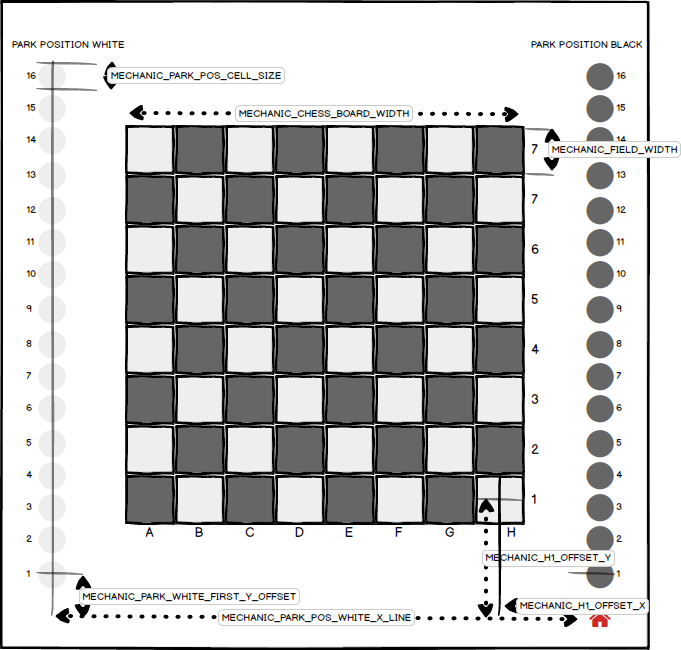
\includegraphics{images/ATC_Calibration_Guide.png}
\caption{Kalibrierungeschema der Mechanik zeigt welche Abstände in der
Konfiguration eigetragen werden müssen}
\end{figure}
